\documentclass{article}

\usepackage{times}
\usepackage{natbib}
\usepackage{amsmath}
\usepackage[pdftex]{graphicx}
\usepackage{sidecap}
\usepackage{hyperref}
\usepackage{float}
\hypersetup{
    colorlinks,%
    citecolor=black,%
    filecolor=black,%
    linkcolor=black,%
    urlcolor=black
}

 

\bibpunct{[}{]}{;}{n}{,}{,}

\newcommand{\BibTeX}{{\sc Bib}\TeX}

\begin{document}
\setlength{\parindent}{0in}%Removing Paragraph Indenting in LaTeX
\author{Behnam Asadi}
\title{Anomaly Detection in Robotic Application Using Gaussian Mixture Model and Kullback-Liebler divergence}
\date{\today}
\maketitle
%\begin{abstract}
%In this paper an effort has been made to detect anomaly in a robot sensor data stream. 
%Our subjected robot is six legged robot named crex, part of the project RIMRES. 
%The evaluated data is current level (in Milliamperes) coming from the joints.
%We propose  an approach for anomaly detection using Gaussian Mixture Model(GMM) and making a comparison between the GMMs by calculating the distance metric between PDFs.
%One of the issues in the  mixture model is to determine the number of components in advance, which considerably impact the outcome and performance. At first we propose a method to find the optimal number of components for GMM and also a rough estimation for other parameters such as weights of components and centers of components, which at the end make the GMM algorithm non-parametric.
%\\
%In the second step, after initializing parameters with outcome that we get from the first step, we have used a well known algorithm called Expectation Maximization(EM) to estimate the values of parameters.
%Then we made a set of robot primitive actions including walking forward/backward, turning right/left, climbing up/down. The system learns normal behavior for these action.
%\\
%In detection phase, the system tries to find the closest pattern to current incoming data by calculating distance metric between PDFs.
%If the distance between incoming data(current) and closest pattern(references behaviors) is more than a given threshold the system would flag that data as anomalous behavior.
%\end{abstract}
%
%{\bf Keywords:} Anomaly Detection in Robots, Gaussian Mixture Model, Pattern Matching, Bayesian Classifier,
%Symmetric Kullback-Liebler
%\section{Introduction}
%Anomalies are the pattern in data that do not conform to a well defined notion of normal data. Application of anomaly detection has been seen is different domains like intrusion detection for cyber security, fraud detection for credit cards,fault detection in safety critical systems etc  \cite{Chandola:2009:ADS:1541880.1541882}.
%
%The importance of anomaly detection is due to the fact that anomalies in data
%translate to significant (and often critical) actionable information in a wide variety of
%application domains \cite{Chandola:2009:ADS:1541880.1541882}. For example, an anomalous traffic pattern in a computer network
%could mean that a hacked computer is sending out sensitive data to an unauthorized
%destination \cite{Parallel_and_distributed_computing_for_cybersecurity}. An anomalous MRI image may indicate presence of malignant tumors
%\cite{991693}. Anomalies in credit card transaction data could indicate credit card or identity theft \cite{618940} or anomalous readings from a space craft sensor could signify a fault in some
%component of the space craft \cite{Fujimaki_2005_ASA_1081870.1081917}.
%
%Various approaches have been used to detect anomalies including supervised and unsupervised techniques and parametric and non parametric systems.\cite{4371451},\cite{Anomaly_Intrusion_Detection_System_Using_Gaussian_Mixture_Model},
%\cite{Anomaly_detection_in_sea_traffic_A_comparison_of_the_Gaussian_Mixture_Model_and_the_Kernel_Density_Estimator},
%\cite{Fully_Unsupervised_Learning_of_Gaussian_Mixtures_for_Anomaly_Detection_in_Hyperspectral_Imagery}
%
%Gaussian Mixture Model(GMM) has been used for anomaly detection in various application such as intrusion detection system(IDS) \cite{Anomaly_Intrusion_Detection_System_Using_Gaussian_Mixture_Model}, sea traffic \cite{Anomaly_detection_in_sea_traffic_A_comparison_of_the_Gaussian_Mixture_Model_and_the_Kernel_Density_Estimator}, Hyperspectral Imagery  \cite{Fully_Unsupervised_Learning_of_Gaussian_Mixtures_for_Anomaly_Detection_in_Hyperspectral_Imagery}.
%
%
%
%
%
%The data that we use in our experiment are sensors data originated from six legged robot.
%The evaluated data is current level (in Milliamperes) coming from the joints.
%\\
%
%%here more info about our data i.e velocity, speed, position, dimension of data, feature space and ... 
%
%%Different types of Anomalies
%
%The rest of this paper is organized as follows:
%Sections \ref{Definition_of_Anomalies} and \ref{Different_types_of_Anomalies}
%give an insight into definition of anomaly and different sort of anomalies.
%In section \ref{Applied_method} our strategy for anomaly detection  has been discussed. In section \ref{Set_of_Normal_Behavior_Patterns} we introduce our set of normal behavior patterns.
%Section \ref{Gaussian_Mixture_Model_and_Expectation_Maximization_Process} introduces Gaussian Mixture Model and Expectation Maximization process in brief and our approach for finding optimal number of components  and section \ref{Comparison_of_Probability_Distribution_Function} discusses 
%our method for making comparison between probability distribution functions.
%Section \ref{Results} is about results. 
%
%\section{Definition of Anomalies}\label{Definition_of_Anomalies}
%Anomalies are patterns in data that do not conform to a well defined notion of normal
%behavior. Figure \ref{AnomalyIllustration}   illustrates anomalies in a simple two-dimensional data set. The data has two normal regions, N1 and N2 , since most observations lie in these two regions.
%Points that are sufficiently far away from these regions, for example, points o1 and o2 ,
%and points in region O3 , are anomalies.
%Anomaly detection has some issues in common with:
%\begin{itemize}
%\item Rare Class Mining 
%\item Chance discovery
%\item Novelty Detection
%\item Exception Mining
%\item Noise Removal
%\end{itemize}
%Anomaly detection is related to, but distinct from noise removal and
%noise accommodation, both of which deal with unwanted
%noise in the data. Noise can be defined as a phenomenon in data that is not of interest
%to the analyst, but acts as a hindrance to data analysis. Noise removal is driven by
%the need to remove the unwanted objects before any data analysis is performed. Noise
%accommodation refers to immunizing a statistical model estimation against anomalous
%observations.
%Another topic related to anomaly detection is novelty detection, which aims at detecting previously unobserved
%(emergent, novel) patterns in the data, for example, a new topic of discussion in a news
%group. The distinction between novel patterns and anomalies is that the novel patterns
%are typically incorporated into the normal model after being detected.
%It should be noted that solutions for these related problems are often used for anomaly
%detection and vice versa \cite{Chandola:2009:ADS:1541880.1541882}.
%
%
%\begin{figure}[H]
%\begin{center}
%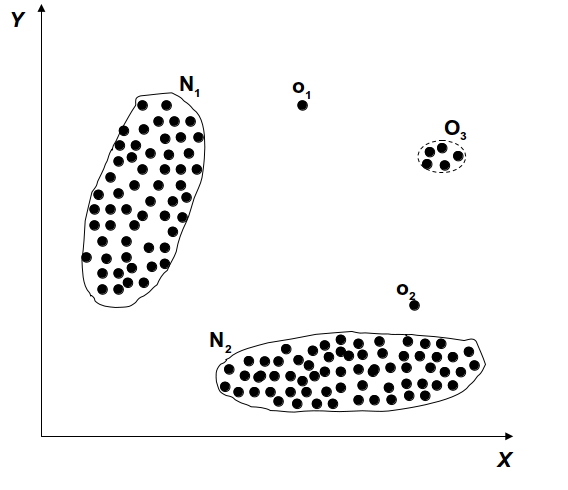
\includegraphics[scale=0.3]{./images/anomaly_illustration.png}
%\caption{A simple example of anomalies in a two-dimensional data set.}
%\label{AnomalyIllustration}
%\end{center}
%\end{figure}
%
%
%\section{Different types of Anomalies}\label{Different_types_of_Anomalies}
%An important aspect of an anomaly detection technique is the nature of the desired
%anomaly. Anomalies can be classified into following three categories\cite{Chandola:2009:ADS:1541880.1541882}:
%\begin{itemize}
%\item Point Anomalies
%\item Contextual Anomalies
%\item Collective Anomalies
%\end{itemize}
%\subsection{Point Anomalies}
%If an individual data instance can be considered as anomalous
%with respect to the rest of data, then the instance is termed a point anomaly. This is the
%simplest type of anomaly and is the focus of majority of research on anomaly detection.
%For example, in Figure \ref{AnomalyIllustration} , points o1 and o2 , as well as points in region O3 , lie outside the boundary of the normal regions, and hence are point anomalies since they are
%different from normal data points.
%As a real-life example, consider credit card fraud detection. Let the data set correspond to an individual’s credit card transactions. For simplicity, let us
%assume that the data is defined using only one feature: amount spent. A transaction
%for which the amount spent is very high compared to the normal range of expenditure
%for that person will be a point anomaly.
%
%\subsection{Contextual Anomalies}
%
%If a data instance is anomalous in a specific context, but
%not otherwise, then it is termed a contextual anomaly (also referred to as conditional
%anomaly [Song et al. 2007]). Figure \ref{Contextual_Anomalies.png} illustrate en example of contextual anomalies,
%The notion of a context is induced by the structure in the data set and has to be
%specified as a part of the problem formulation. Each data instance is defined using the
%following two sets of attributes:
%\begin{itemize}
%\item Contextual attributes
%
%The contextual attributes are used to determine the context
%(or neighborhood) for that instance. For example, in spatial data sets, the longitude
%and latitude of a location are the contextual attributes. In time-series data, time
%is a contextual attribute that determines the position of an instance on the entire
%sequence.
%
%\item Behavioral attributes
%
%The behavioral attributes define the noncontextual characteristics of an instance. For example, in a spatial data set describing the average rainfall of the entire world, the amount of rainfall at any location is a behavioral
%attribute. 
%\end{itemize}
%
%\begin{figure}[H]
%\begin{center}
%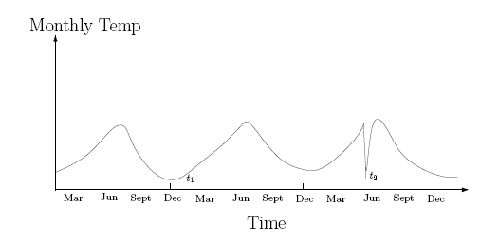
\includegraphics[scale=0.7]{./images/Contextual_Anomalies.png}
%\caption{Contextual anomaly t2 in a temperature time-series. Note that the temperature at time t1 is same as that at time t2 but occurs in a different context and hence is not considered as an anomaly.}
%\label{Contextual_Anomalies.png}
%\end{center}
%\end{figure}
%
%
%
%
%\subsection{Collective Anomalies}
%If a collection of related data instances is anomalous with
%respect to the entire data set, it is termed a collective anomaly. The individual data
%instances in a collective anomaly may not be anomalies by themselves, but their occurrence together as a collection is anomalous. Figure \ref{Collective_Anomalies.png} 
% is an example that shows a human
%electrocardiogram output \cite{PhysioNet}. The highlighted region denotes an
%anomaly because the same low value exists for an abnormally long time (corresponding to an Atrial Premature Contraction). Note that that low value by itself is not an anomaly
%\begin{figure}[H]
%\begin{center}
%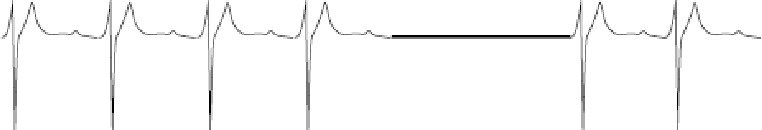
\includegraphics[scale=0.4]{./images/Collective_Anomalies.png}
%\caption{Collective anomaly corresponding to an Atrial Premature Contraction in an human electrocardiogram output.}
%\label{Collective_Anomalies.png}
%\end{center}
%\end{figure}
%
%\section{Description of Applied method and Motivation}\label{Applied_method}
%The whole idea in our technique for detecting anomaly behavior is to compare the probability density function of incoming data with our set normal behavior for walking, climbing and turning, with different parameters and values. First we try to find the closet pattern to our incoming data and then we measure the distance. If the distance is more than a given threshold, we would call that data anomalous behavior.
%\\
%To approximate the probability distribution of our data, we have used  Gaussian Mixture Model (GMM)
%The motivations for using GMM are lack of knowledge about distribution of data and robustness of GMM model to approximate any probability distribution with arbitrary accuracy.
%Gaussian Mixture Model has been described in section \ref{gmm}.
%\\
%One of the issues in the  mixture model is to determine number of components in advance, which considerably impact the outcome and performance. We propose a method to find optimal number of components for GMM and also a rough estimation for other parameters such as weights of components and centers of components.
%These method has been discussed fully in sections \ref{k-means}, \ref{ClusterValidation} and \ref{ParameterInitialization}.
%\\
%In the next step, after initializing parameters with outcome that we get form previous step, we have used a well known algorithm called Expectation Maximization(EM) to estimate the values of parameters and make the pdf of normal behavior for walking climbing turning.
%\\
%In detection phase, the system would try to find the closest pattern to current incoming data by calculating distance metric between PDFs.
%if the distance between incoming data(current) and closest pattern(references behaviors) is more than a given threshold the system would flag that data as anomalous behavior.
%
%\section{Set of Normal Behavior Patterns }\label{Set_of_Normal_Behavior_Patterns}
%Our initial training set consist of sensory data coming from the robot in different situation, with different parameters.In our training set we had set of pattern for walking forward/backward, turning right/left, climbing up/down with different values for speed and angles of legs.
%
%\section{Gaussian Mixture Model and Expectation Maximization Process}
%\label{Gaussian_Mixture_Model_and_Expectation_Maximization_Process}
%The GMM is a robust parametric density model used for approximating a
%A Gaussian mixture density is a weighted sum of K component densities with the equation given by  \ref{eq:MixtureOfGaussians}, We therefore consider a superposition of K Gaussian densities of the form
%
%\begin{equation} \label{eq:MixtureOfGaussians}
%P(X|\lambda)=\sum_{k=1}^{K}\pi_{k}\mathcal{N}_{k}(X|\mu_{K},\Sigma_{k})
%\end{equation}
%
%which is called a mixture of Gaussians. Each Gaussian density \( \mathcal{N}_{k}(X|\mu_{K},\Sigma_{k}) \)
%is called a component of the mixture and has its own mean \(\mu_{K} \) and covariance \(\Sigma_{k}\) and X is D-Dimensional vector.
%By using a sufficient number of Gaussians, and by adjusting their
%means and covariances as well as the coefficients in the linear combination, almost
%any continuous density can be approximated to arbitrary accuracy \cite{Pattern_Recognition_and_Machine_Learning}.
%
%The parameters \( \pi_{K} \) are called mixing coefficients (or weights). If we integrate both
%sides, with respect to x, and note that both \( P(X) \)  and the individual Gaussian components are normalized, we obtain
%
%\begin{equation} \label{eq:SumOfWeights}
%\sum_{k=1}^{K}\pi_{k}=1
%\end{equation}
%
%Also, the requirement that \( P(X) \geq 0 \), together with \( \mathcal{N}_{k}(X|\mu_{K},\Sigma_{k}) \geq 0  \), \( \pi_{k} \geq 0 \) for all k. Combining this with the condition \ref{eq:SumOfWeights} we obtain \( 0\leq \pi_{k} \leq 1 \). We therefore see that the mixing coefficients satisfy the requirements to be probabilities. From the sum and product rules, the marginal density is given by:
%\begin{equation} \label{eq:SumOfWeights}
%p(X)=\sum_{k=1}^{K}p(k)p(X|k).
%\end{equation}
%which is equivalent to \ref{eq:MixtureOfGaussians} in which we can view \( \pi_{k}= p(k)\) as the prior probability of picking the \( k_{th} \) component, and the density
% \( \mathcal{N}_{k}(X|\mu_{k},\Sigma_{k})=P(X|k)  \) as the probability of x conditioned on k 
%\cite{Pattern_Recognition_and_Machine_Learning}.
%Gaussian function for D-Dimensional variate X, for \(k_{th}\) component  is in the form of:
%\[
%\mathcal{N}_{k}(X)=\frac{1}{(2\pi)^{D/2}|\Sigma_{k}|^{1/2}}exp{-\frac{1}{2}(X-\mu_{k})^{T}\Sigma_{k}^{-1}(X-\mu_{k})}
%\]
%The complete Gaussian mixture density is parametrized by the mean vectors, covariance matrices and mixture weights. These parameters are collectively represented by the notation:
%\( \lambda=\{\pi_{k},\mu_{k},\Sigma_{k} \} \) 
%\(k=\{1...K\}\)
%Each class of action (walking forward/backward, turning right/left, climbing up/down) is represented by a GMM and is referred to by a model \(\lambda\).
%\subsection{Covariance matrix}
%Because of assumption of i.i.d (Independent and identically distributed) for our variables, we have used a diagonal matrix as covariance matrix.
%To find the parameters for 
%
%\subsection{K-means algorithm}\label{k-means}
%K-means Clustering is being used for identifying groups, or clusters, of data points in a multidimensional space.
%This is one of the most popular and well-known clustering algorithms. It can be viewed as a special case of the generalized hard clustering algorithmic scheme when point representatives are used and the squared Euclidean distance is adopted to measure the dissimilarity between vectors \(x_{n}\) and cluster representatives \(\mu_{k} \) \cite{theodoridis2009pattern}.
%
%We begin by considering the problem of identifying groups, or clusters, of data points
%in a multidimensional space. Suppose we have a data set \({x1 , . . . , xN } \)consisting
%of N observations of a random D-dimensional Euclidean variable x. Our goal is to
%partition the data set into some number K of clusters, where we shall suppose for
%the moment that the value of K is given. Intuitively, we might think of a cluster as
%comprising a group of data points whose inter-point distances are small compared
%with the distances to points outside of the cluster. We can formalize this notion by
%first introducing a set of D-dimensional vectors \(\mu_{k} \), where \( k = 1, . . . , K, \) in which
%\(\mu_{k} \) is a prototype associated with the \(K_{th} \) cluster. As we shall see shortly, we can
%think of the \(\mu_{k} \) as representing the centers of the clusters. Our goal is then to find
%an assignment of data points to clusters, as well as a set of vectors  \( { \mu_{k} }\) , such that
%the sum of the squares of the distances of each data point to its closest vector \(\mu_{k} \) , is
%a minimum.
%
%
%It is convenient at this point to define some notation to describe the assignment
%of data points to clusters. For each data point \(x_{n} \) , we introduce a corresponding set
%of binary indicator variables \(r_{nk} \in {0, 1} \), where \( k = 1, . . . , K \) describing which of
%the K clusters the data point \(x_{n}\) is assigned to, so that if data point \(x_{n}\) is assigned to
%cluster k then \(r_{nk} = 1 \), and \(r_{nj}\) = 0 for j = k. This is known as the 1-of-K coding
%scheme. We can then define an objective function, sometimes called a distortion
%measure, given by:
%
%\begin{equation} \label{eq:K-means}
%J=\sum_{n=1}^{N}\sum_{k=1}^{K} r_{nk} | x_{n} -\mu_{k}|^{2}
%\end{equation}
%which represents the sum of the squares of the distances of each data point to its
%assigned vector \(\mu_{k} \). Our goal is to find values for the \( {r_{nk} } \)and the \( { \mu_{k} } \)so as to minimize J. We can do this through an iterative procedure in which each iteration
%involves two successive steps corresponding to successive optimizations with respect
%to the \( r_{nk}\) and the \( \mu_{k} \). First we choose some initial values for the \(\mu_{k}\) . Then in the first phase we minimize J with respect to the \(r_{nk}\) , keeping the \(\mu_{k}\) fixed. In the second phase we minimize J with respect to the \(\mu_{k} \) , keeping \(r_{nk}\) fixed. This two-stage optimization is then repeated until convergence \cite{Pattern_Recognition_and_Machine_Learning423}.
%
%\subsection{Cluster Validation}\label{ClusterValidation}
%In order to find the optimal number of components for GMM, first we used k-means algorithm with different number of clusters (starting from 1 to a fixed number), then we checked the cluster validity by deploying the C-index (\citet*{c-index}) algorithm and select the optimal number of clusters with lowest C-index.
%This index is defined as follows:
%(Hubert and Schultz, 1976)
%
%\[ C=\frac{S-S_{min}}{{S_{max}-S_{min}}} \]
%
%where S is the sum of distances over all pairs of patterns from the same cluster. Let l be the number of those pairs. Then \( S_{min} \) is the sum of the \emph{l}  smallest distances if all pairs of patterns are considered (i.e. if the patterns can belong to different clusters). Similarly \(S_{max}\)  is the sum of the  \emph{l} largest distance out of all pairs. Hence a small value of C indicates a good clustering.
%
%
%We also used the centroids of the selected cluster as initial parameter for means in Expectation Maximization algorithm. Furthermore 
%\[ 
%\frac{Number\: of\: data\: points\: in\: cluster}{Total\: number\: of\: data\: points} 
%\] 
%as an initial parameter for the Weights of components.
%\subsection{Parameter Initialization}\label{ParameterInitialization} 
%One drawback of EM(Expectation Maximization) for GMM model is determining number of components in advance. Theoretically there is no way to estimate the number of components. Selecting too few components would result in inaccurate, poor model which doesn’t accurately describe the real data.
%While selecting large number for components, would increase the complexity and computation in both training and test phase. 
%\\
%The initialization of parameters for EM algorithm has massive impact on the result. Different initialization might converge to different local maxima of the likelihood function.\cite{Anomaly_Intrusion_Detection_System_Using_Gaussian_Mixture_Model}
%We use the number of clusters as optimal number of component for GMM. Furthermore we use centers of the clusters as initial parameter for means and number of data points in each cluster over total number of data points as weight of each cluster.
%


\section{Comparison of Probability Distribution Function}\label{Comparison_of_Probability_Distribution_Function}
In the detection phase, in order to find closest pattern to incoming data, the PDF corresponding to each pattern of walking including: walking forward/backward, turning right/left, climbing up/down with different values for speed and angles of legs is compared with incoming data, and the pattern closest to  that would returned as result. This step suggests that we must use some distance metric to compare PDFs. There is no universally accepted such distance metric \cite{Introduction_to_Statistical_Pattern_Recognition}. Two commonly used metrics for measuring PDF distances are the Kullback-Liebler divergence and the Bhattacharyya distance.
\citet{An_Analytic_Distance_Metric_for_Gaussian_Mixture_Models} have proposed a new 
 distance metric that leads to an analytical formula in the case where the
probability density functions correspond to Gaussian Mixtures.

If the distance between incoming data (current) and closest pattern (references behaviors) is more than a given threshold the system would flag that data as anomalous behavior.

One way to calculate the distance between two PDFs \( p(x)\) and \(p^{\prime}(x) \), is the Kullback-Liebler divergence \cite{Introduction_to_Statistical_Pattern_Recognition}.



\begin{equation} \label{Kullback_Liebler_divergence}
D_{KL}(p||p^{\prime})=\int_{-\infty}^\infty p(x)\log\frac{p(x)}{p^{\prime}(x)}  \,\mathrm{d}x
\end{equation}
which could be used to calculate the distance between two arbitrary distribution including two Gaussians, but in our case we have a mixture of Gaussians for each distribution and therefore it is not possible to apply the equation. \citet{An_Analytic_Distance_Metric_for_Gaussian_Mixture_Models} have extended the Kullback Liebler divergence for GMM and proposed a distance metric using the values \(\mu ,\Sigma,\pi \) for each one of the two distributions in the following form:

\begin{equation} \label{Kullback_Liebler_divergence}
C2(p||p^{\prime})=-\log \large[ \frac{2\sum_{i,j}\pi_{i}\pi_{j}^{\prime} \sqrt{ \frac{|V_{ij}|}{e^{k_{ij}}|\sum_{i}| |\sum_{j}^{\prime}|} }  }
%denominator
{
%left part
\sum_{i,j}\pi_{i}\pi_{j} \sqrt{ \frac{|V_{ij}|}{e^{k_{ij}}|\sum_{i}| |\sum_{j}|} }+
%right part
\sum_{i,j}\pi_{i}^{\prime}\pi_{j}^{\prime} \sqrt{ \frac{|V_{ij}|}{e^{k_{ij}}|\sum_{i}^{\prime}| |\sum_{j}^{\prime}|} }
} 
\large]
\end{equation}
Where:
\begin{equation}\label{Kullback_Liebler_divergence_Details1}
V_{ij}=(\Sigma_{i}^{-1} +\Sigma_{j}^{-1})^{-1}
\end{equation}
and
\begin{equation}\label{Kullback_Liebler_divergence_Details2}
K_{ij}=\mu_{i}^{T}\Sigma_{i}^{-1}(\mu_{i}-\mu_{j}^{\prime})+\mu_{j}^{\prime T}\Sigma_{j}^{\prime -1}(\mu_{j}^{\prime}-\mu_{i})
\end{equation}
\section{Results}\label{Results}
%\section{Future Works}\label{Future_Works}
%\section{Limitations}\label{Limitations}






%Due to the fact that we don't know the structure of coming data from RIMRES sensors, we assume that it is normal and we tried to fit the data with mixture of Gaussian distribution, with unknown parameters.
%These parameters are  weight, mean and standard deviation for each one them.
%We also need to determine number of  Gaussian distributions 
%To find the optimal number of Gaussian, I found several methods:
%1. starting with 1 component and then increasing that and use hold out method to determine when we are starting over-fit the data
%2. Using Bayesian framework.
%And the other one which  I develop one by my own.   
%In my approach I used k-means  clustering with one component, and gradually increasing number of components. To validate clusters, I used c-index(smaller c-index, better clustering)
%After I found the optimal number of clusters, I also used centroid and number of items in each cluster s for initialization of  of mean and weight in Expectation maximization model.
%
%After finding optimal number of components and their parameter,that we have to find the closest pattern from our training set to our incoming data.
%
%
% our training set consist of different classes, both for normal and anomaly data, for instance in an IDS system, the network traffic has normal traffic, DOS attack, Probe attack and …
%In my experiments I have used the second approach. But the problem is we don't have any pattern for anomaly behavior(we don’t have any pdf for anomalous data), so for training set I created basic movements for RIMRES robot, i.e.  walking, turning to right/left, climbing up/down … and then we compare robot sensors data to these classes and try to find the one which closer to it. Then we would check how close is this pattern to its class(what is the distance between observed data and it's class, i.e. our system has detected that the closest pattern to observed data is climbing up, then we check distance between observed data and climbing up, if it was bigger than a threshold then it is anomaly).
\bibliographystyle{plainnat}
\bibliography{references}

\end{document}